\subsection{Tunneln durch eine Potentialbarriere}
	\begin{align*}
		V(x) = \lambda(x^2- a^2)^2
	\end{align*}
	\begin{figure}
		\begin{center}
			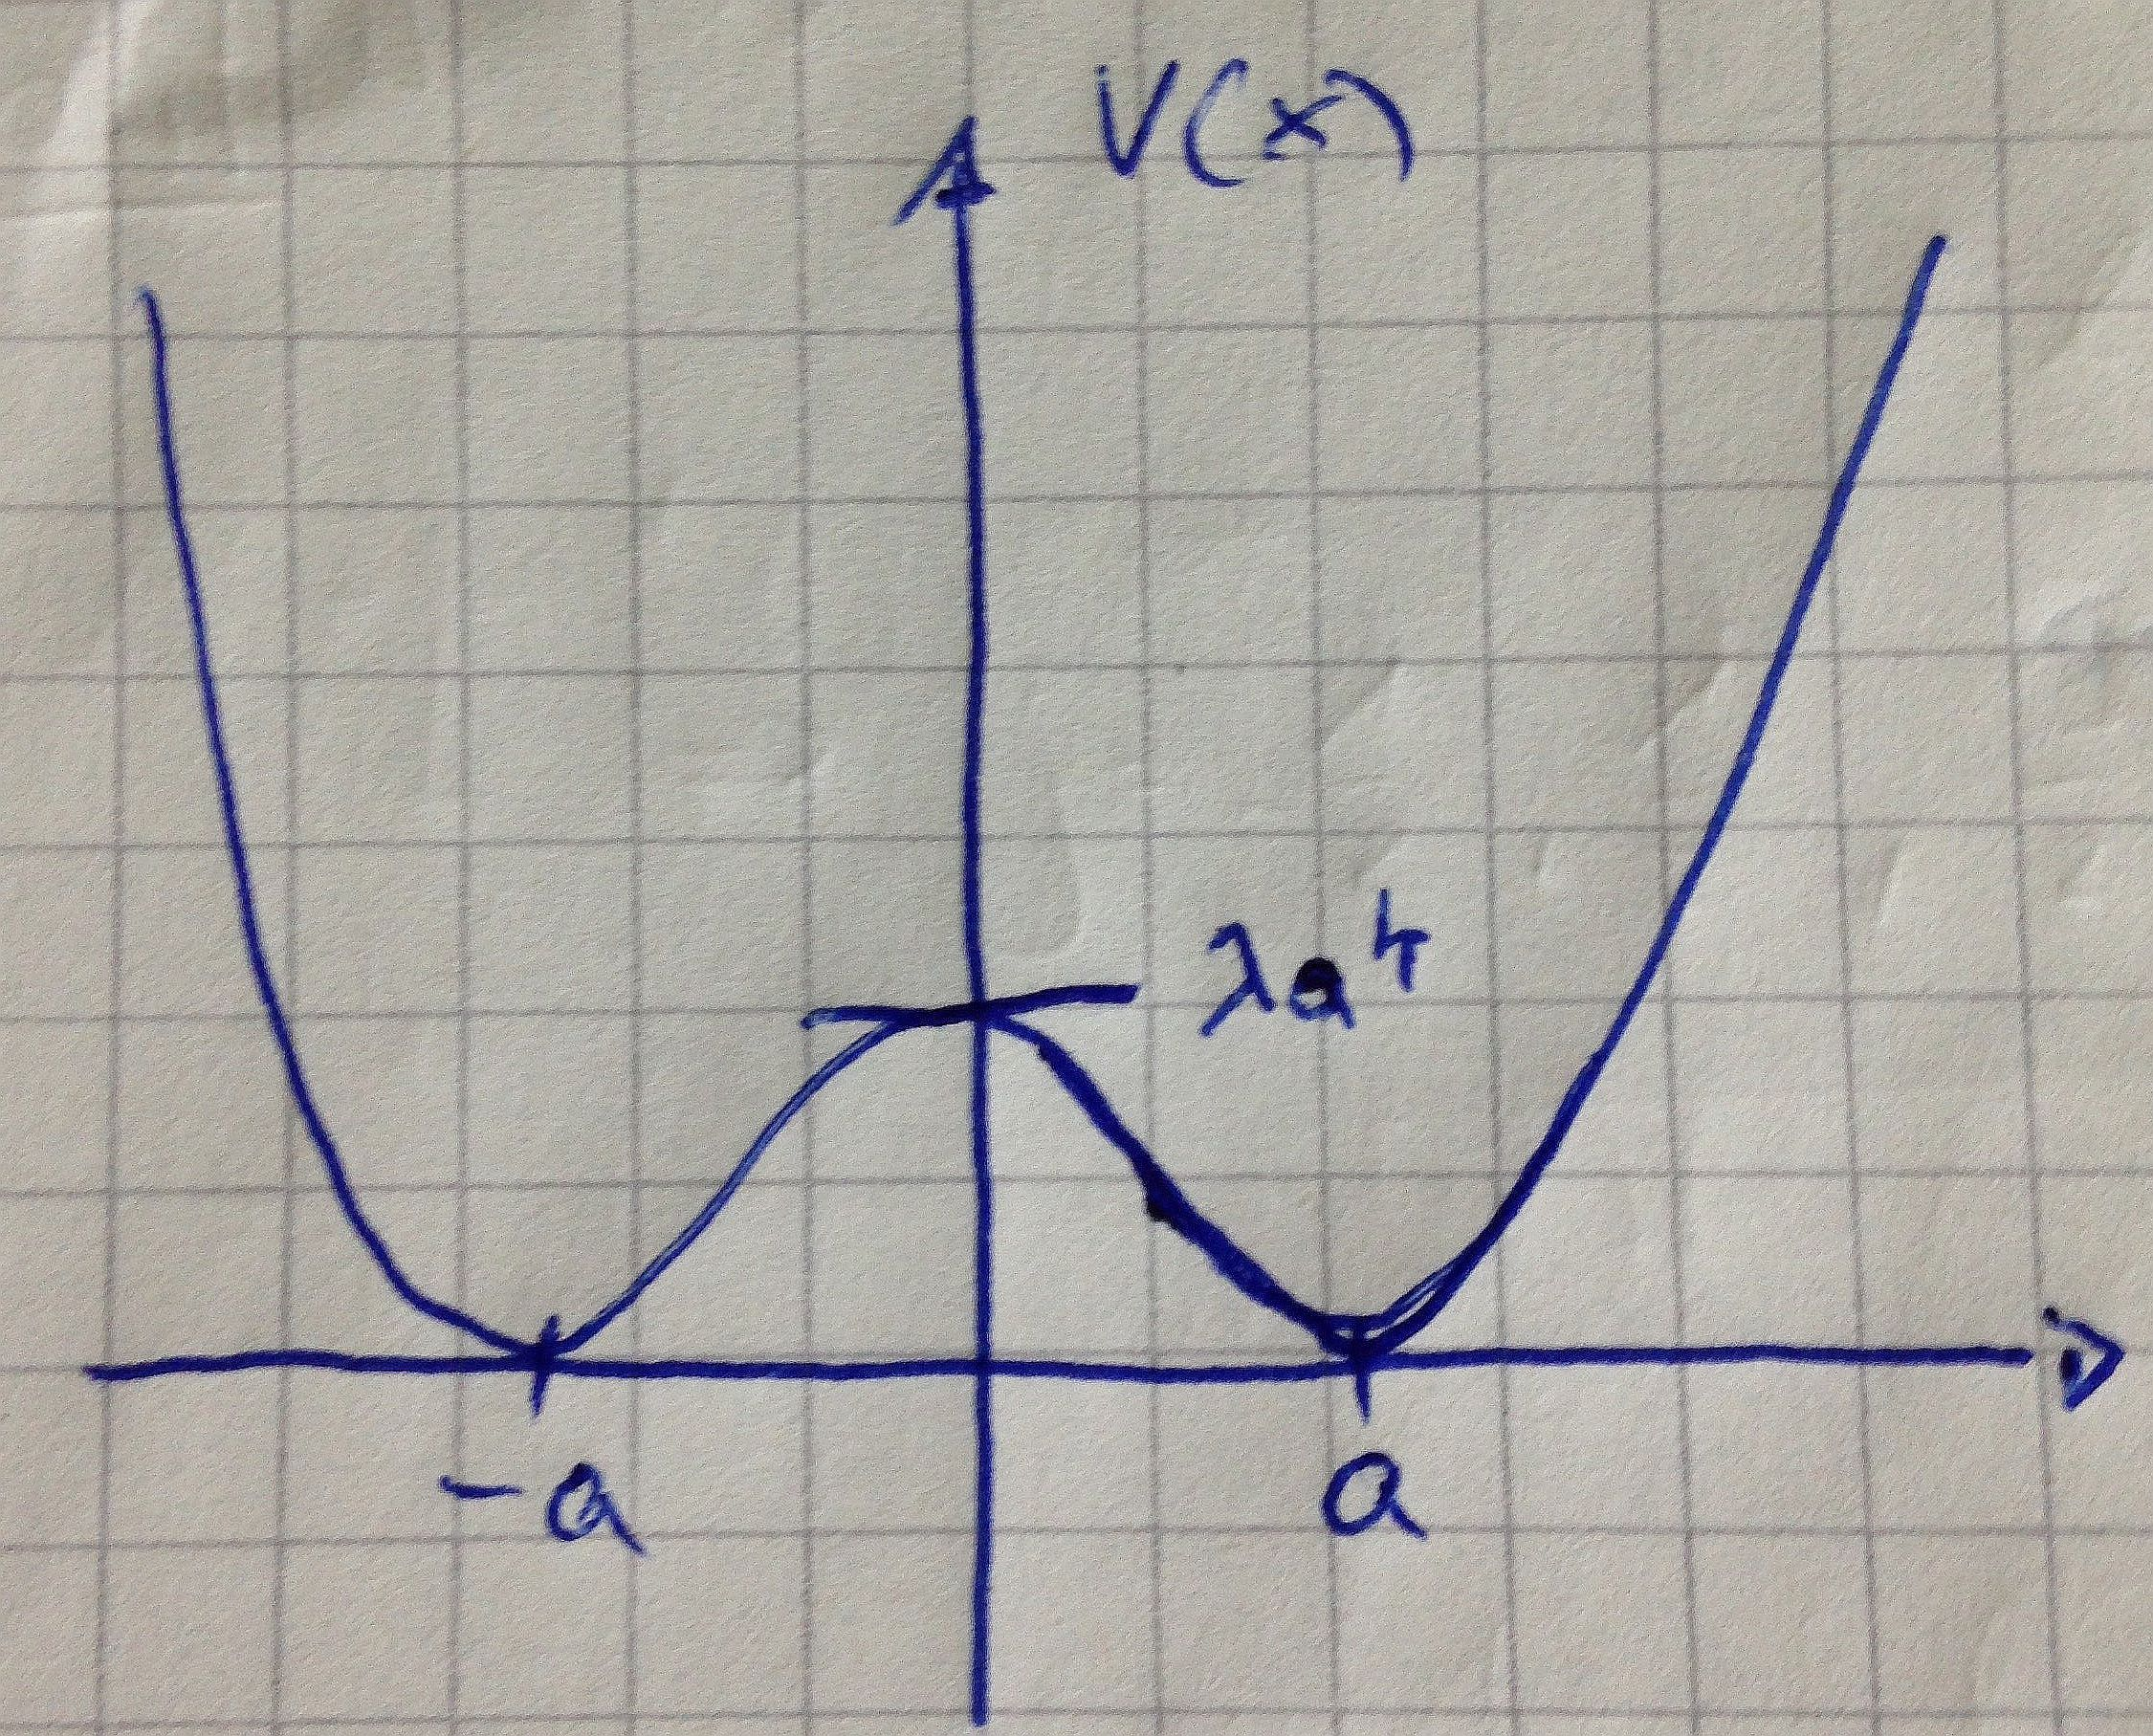
\includegraphics[width= 0.5\textwidth]{Tunneln_durch_eine_Potentialbarriere1}
		\end{center}
	\end{figure}
\FloatBarrier
Grundzustand $\ket{0}$ (symmetrische Wellenfunktion)
\FloatBarrier
	\begin{figure}[h]
		\begin{center}
			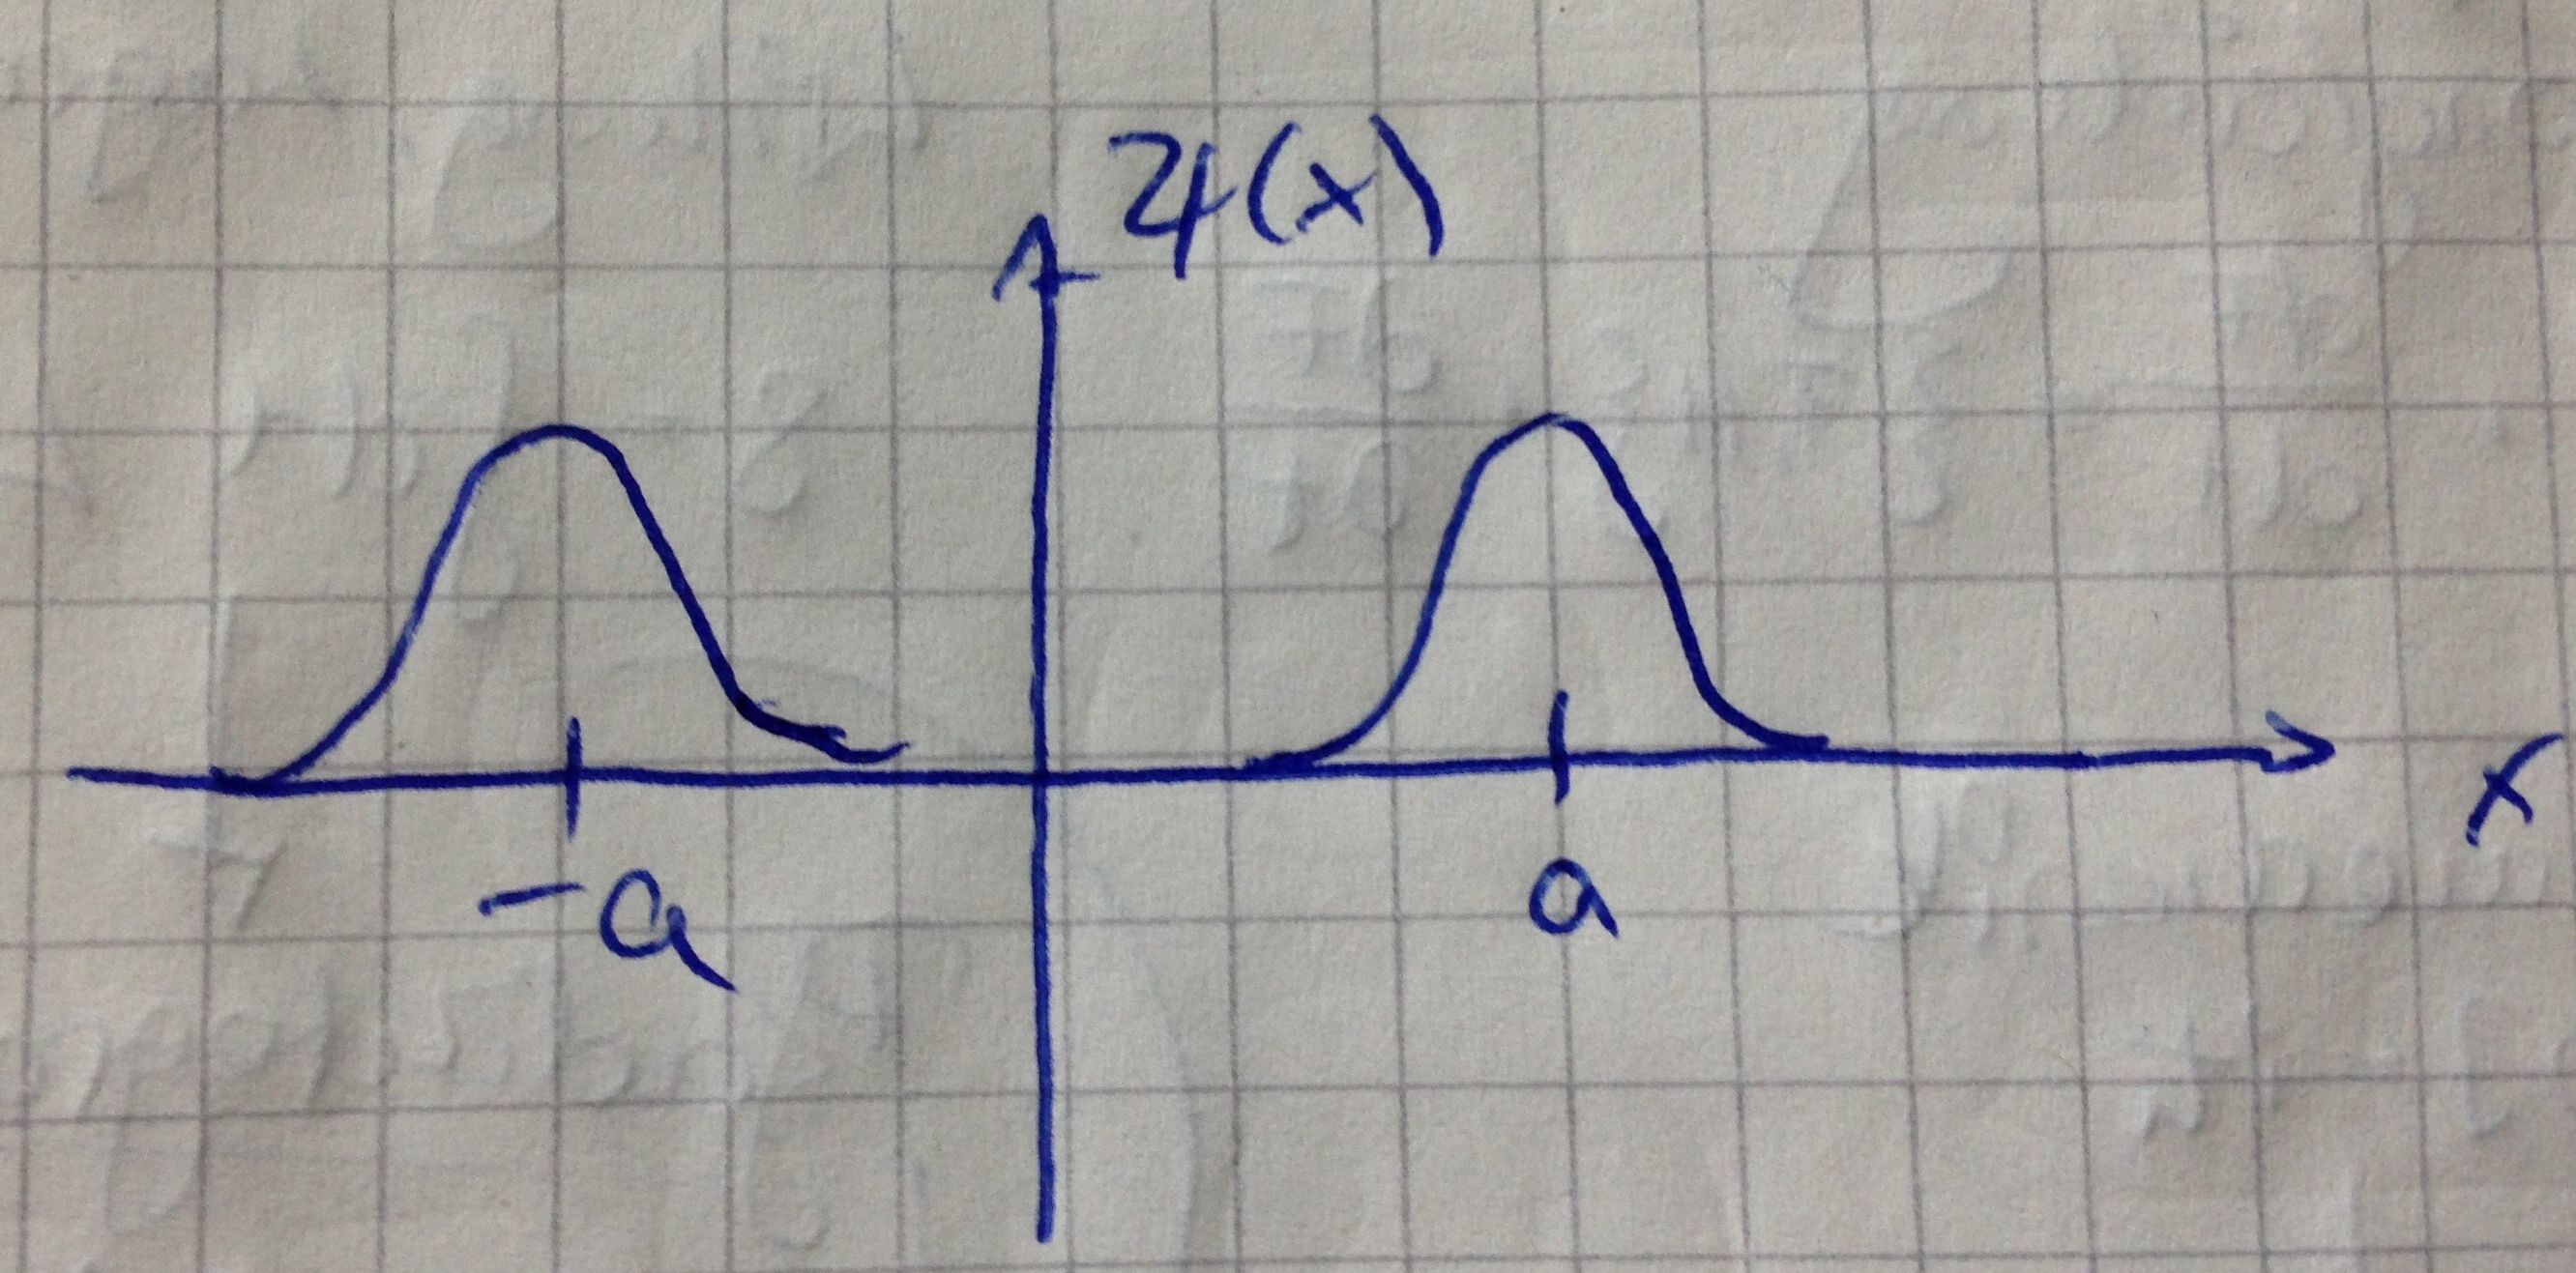
\includegraphics[width= 0.5\textwidth]{Tunneln_durch_eine_Potentialbarriere2}
		\end{center}
	\end{figure}
1. Anregung $\ket{1}$
	\begin{figure} [h]
		\begin{center}
			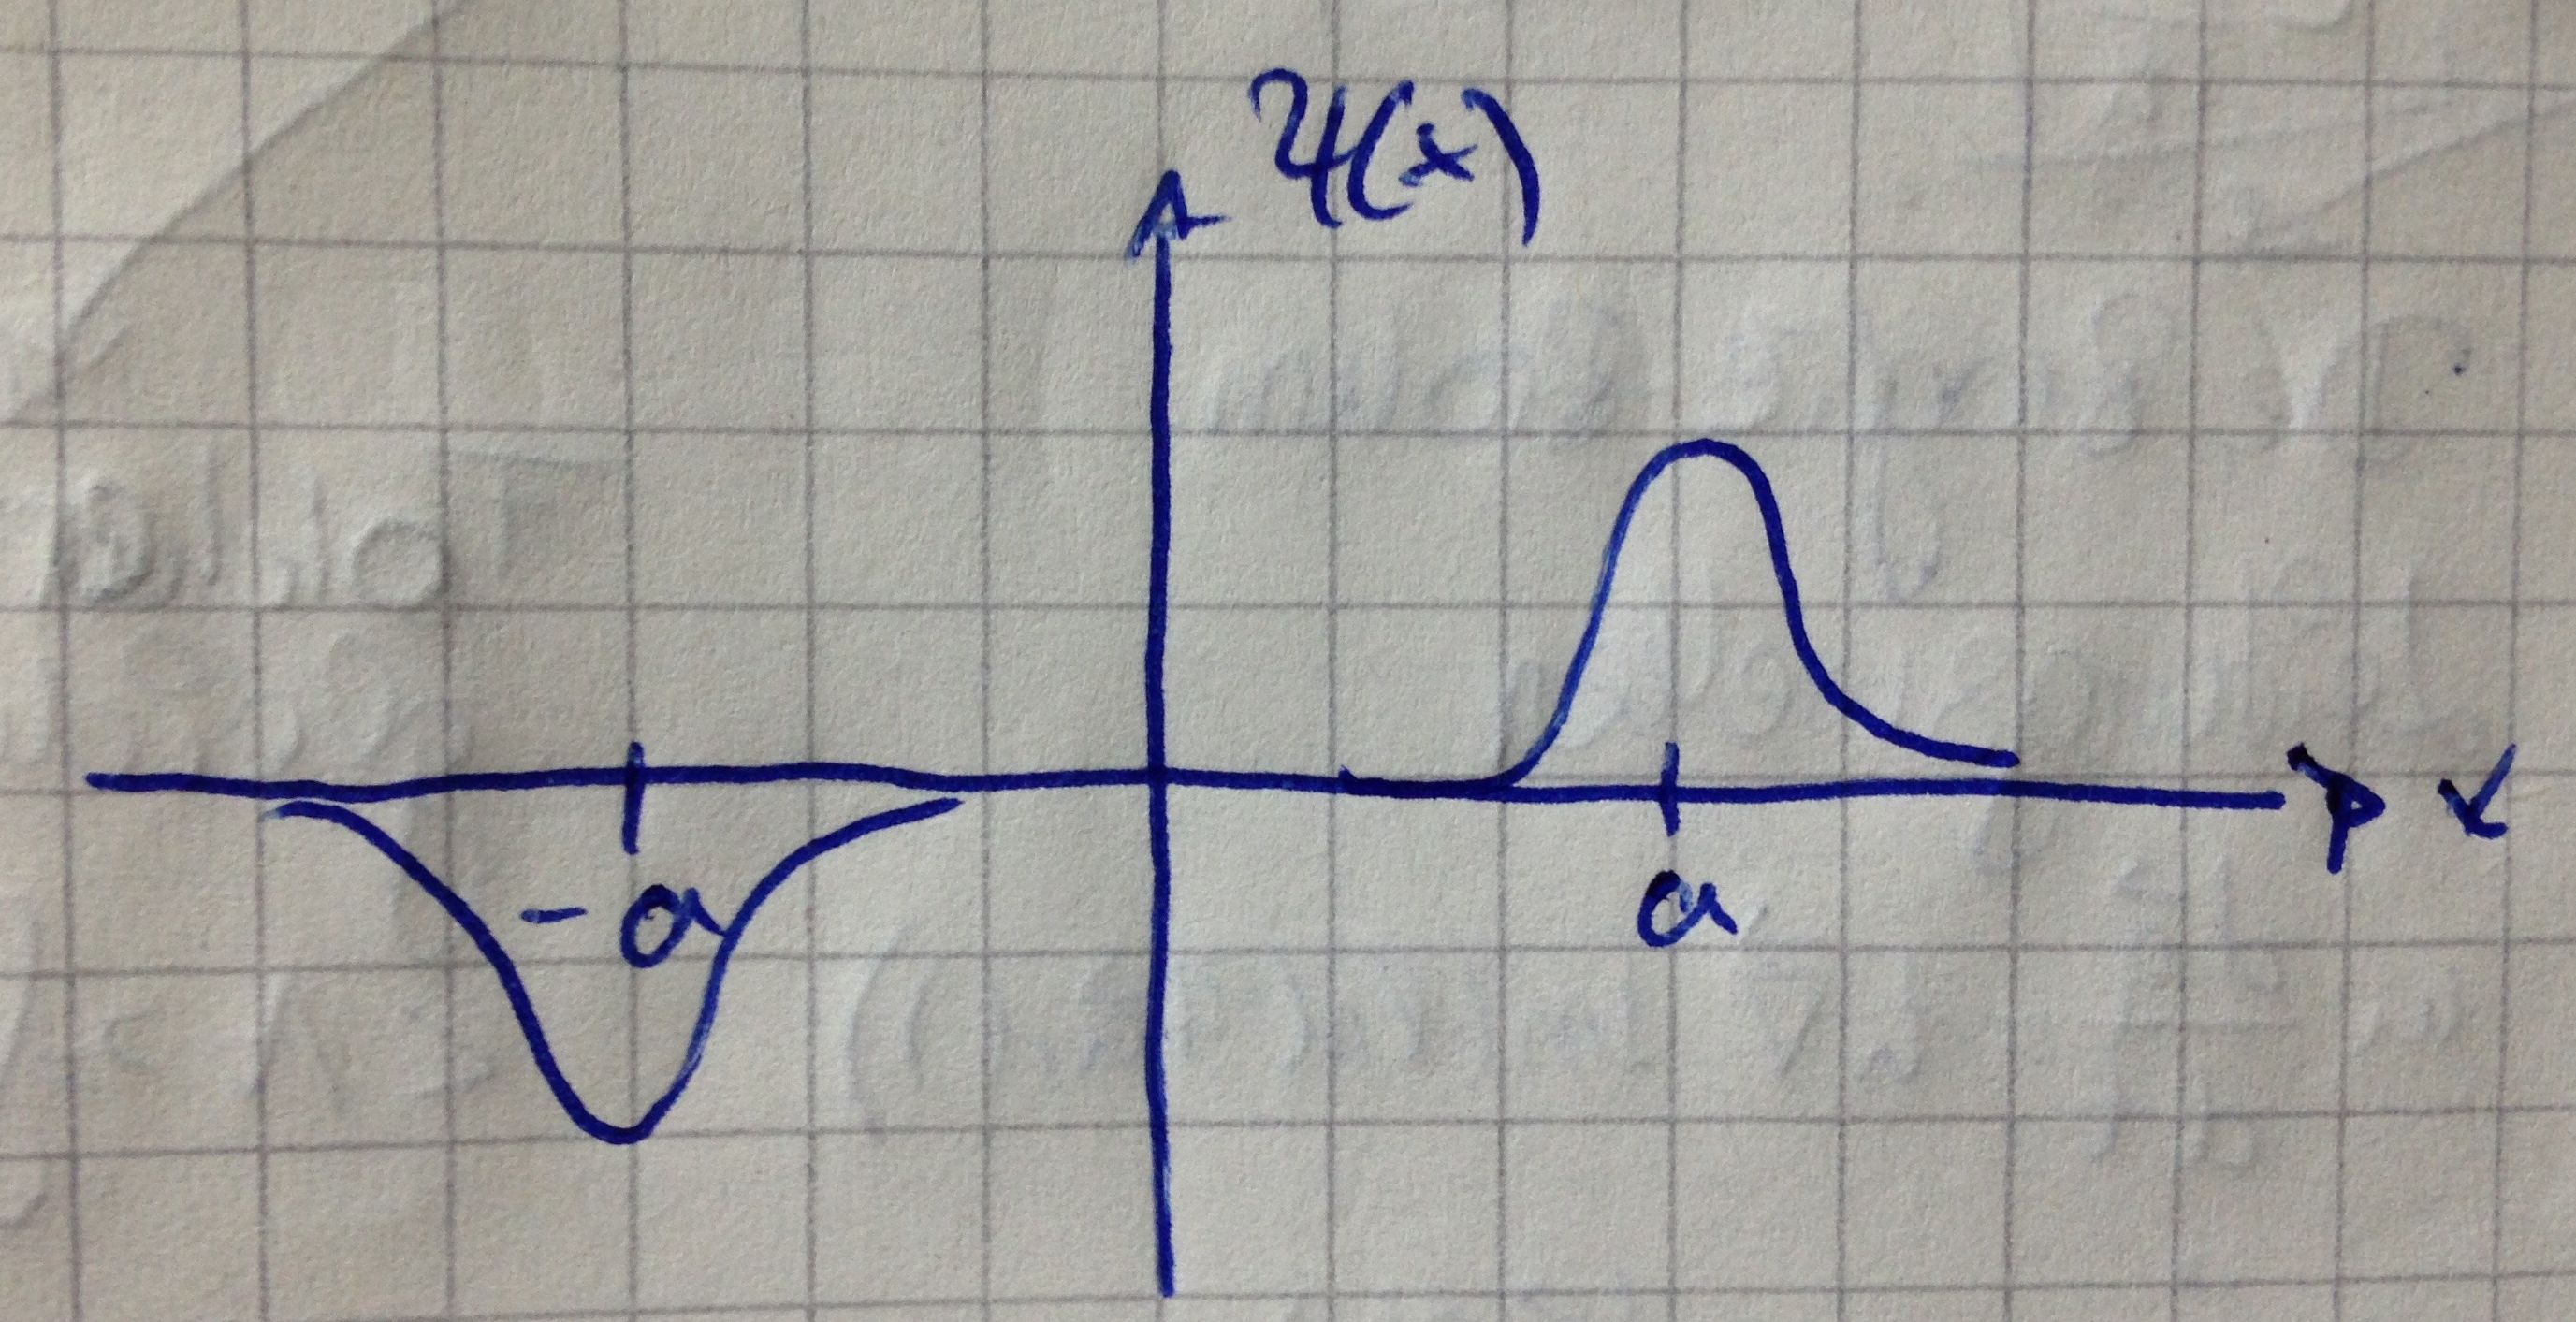
\includegraphics[width= 0.5\textwidth]{Tunneln_durch_eine_Potentialbarriere3}
		\end{center}
	\end{figure}
\FloatBarrier
\newpage
Definiere $\ket{+}$	und $\ket{-}$
	\begin{figure} [h]
		\begin{center}
			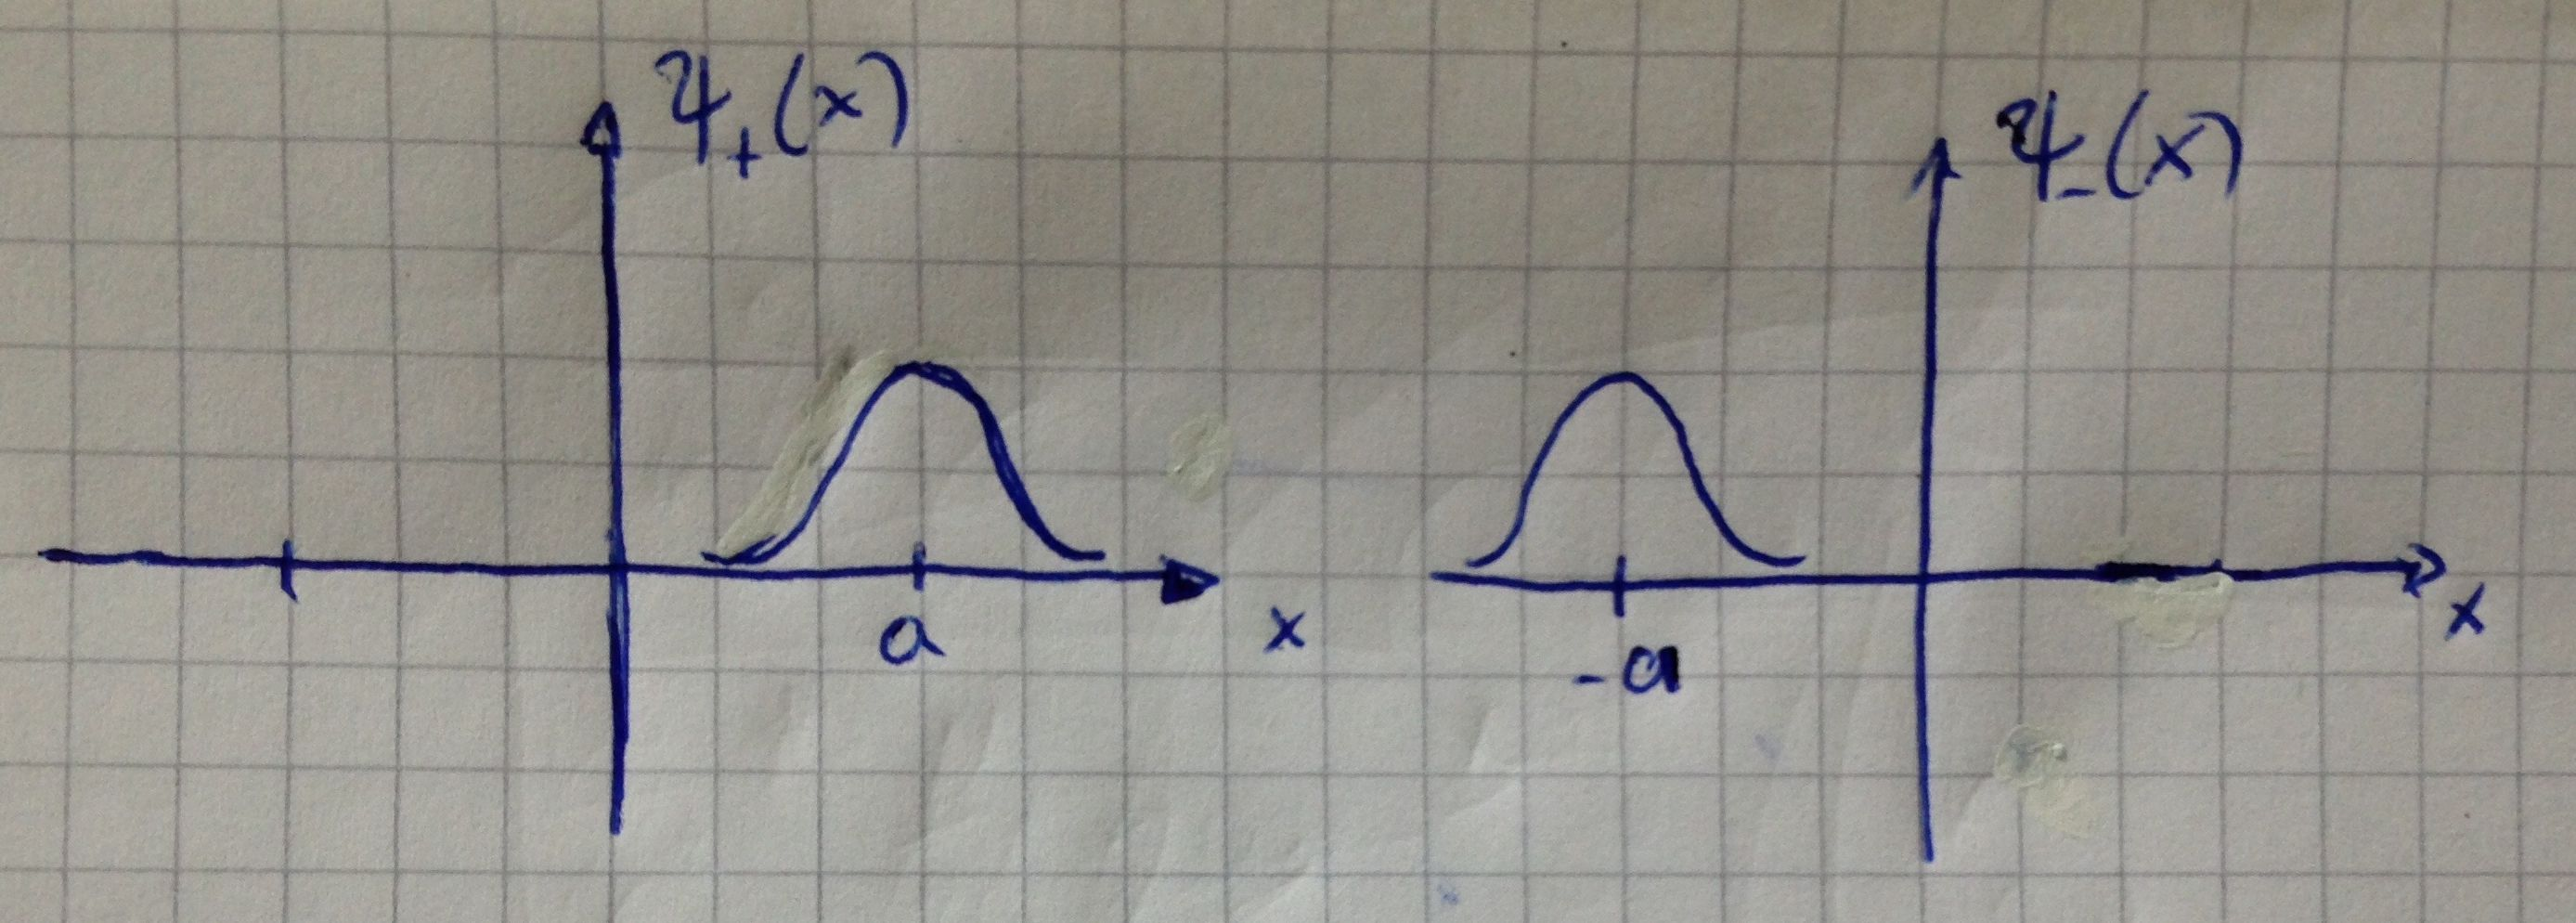
\includegraphics[width= \textwidth]{Tunneln_durch_eine_Potentialbarriere4}
		\end{center}
	\end{figure}
\FloatBarrier
	\begin{align*}
		\ket{0} &\approx \frac{1}{\sqrt{2}} \left(\ket{+} + \ket{-}\right) \\
		\ket{1} &\approx \frac{1}{\sqrt{2}} (\ket{+} - \ket{-}) \\
		\Delta E &= E_1 - E_0 > 0 
	\end{align*}
Beispiel: Amoniak maser

Tunnelprozesse:
	\begin{align*}
		S_E &= \int \limits_{-\frac{T}{2}}^{\frac{T}{2}} \diff \tau 
		\left(\frac{m}{2} \dot{x}^2 + V(x)\right) & \text{ mit Randbedingung:}&\\
		&&x \left(-\frac{T}{2}\right) &= -a ,~ x \left(\frac{T}{2}\right) = a \\
		\braket{+ | -} &= \int [\diff x] e^{-S_E[x]}
	\end{align*}
	\begin{figure} [h]
		\begin{center}
			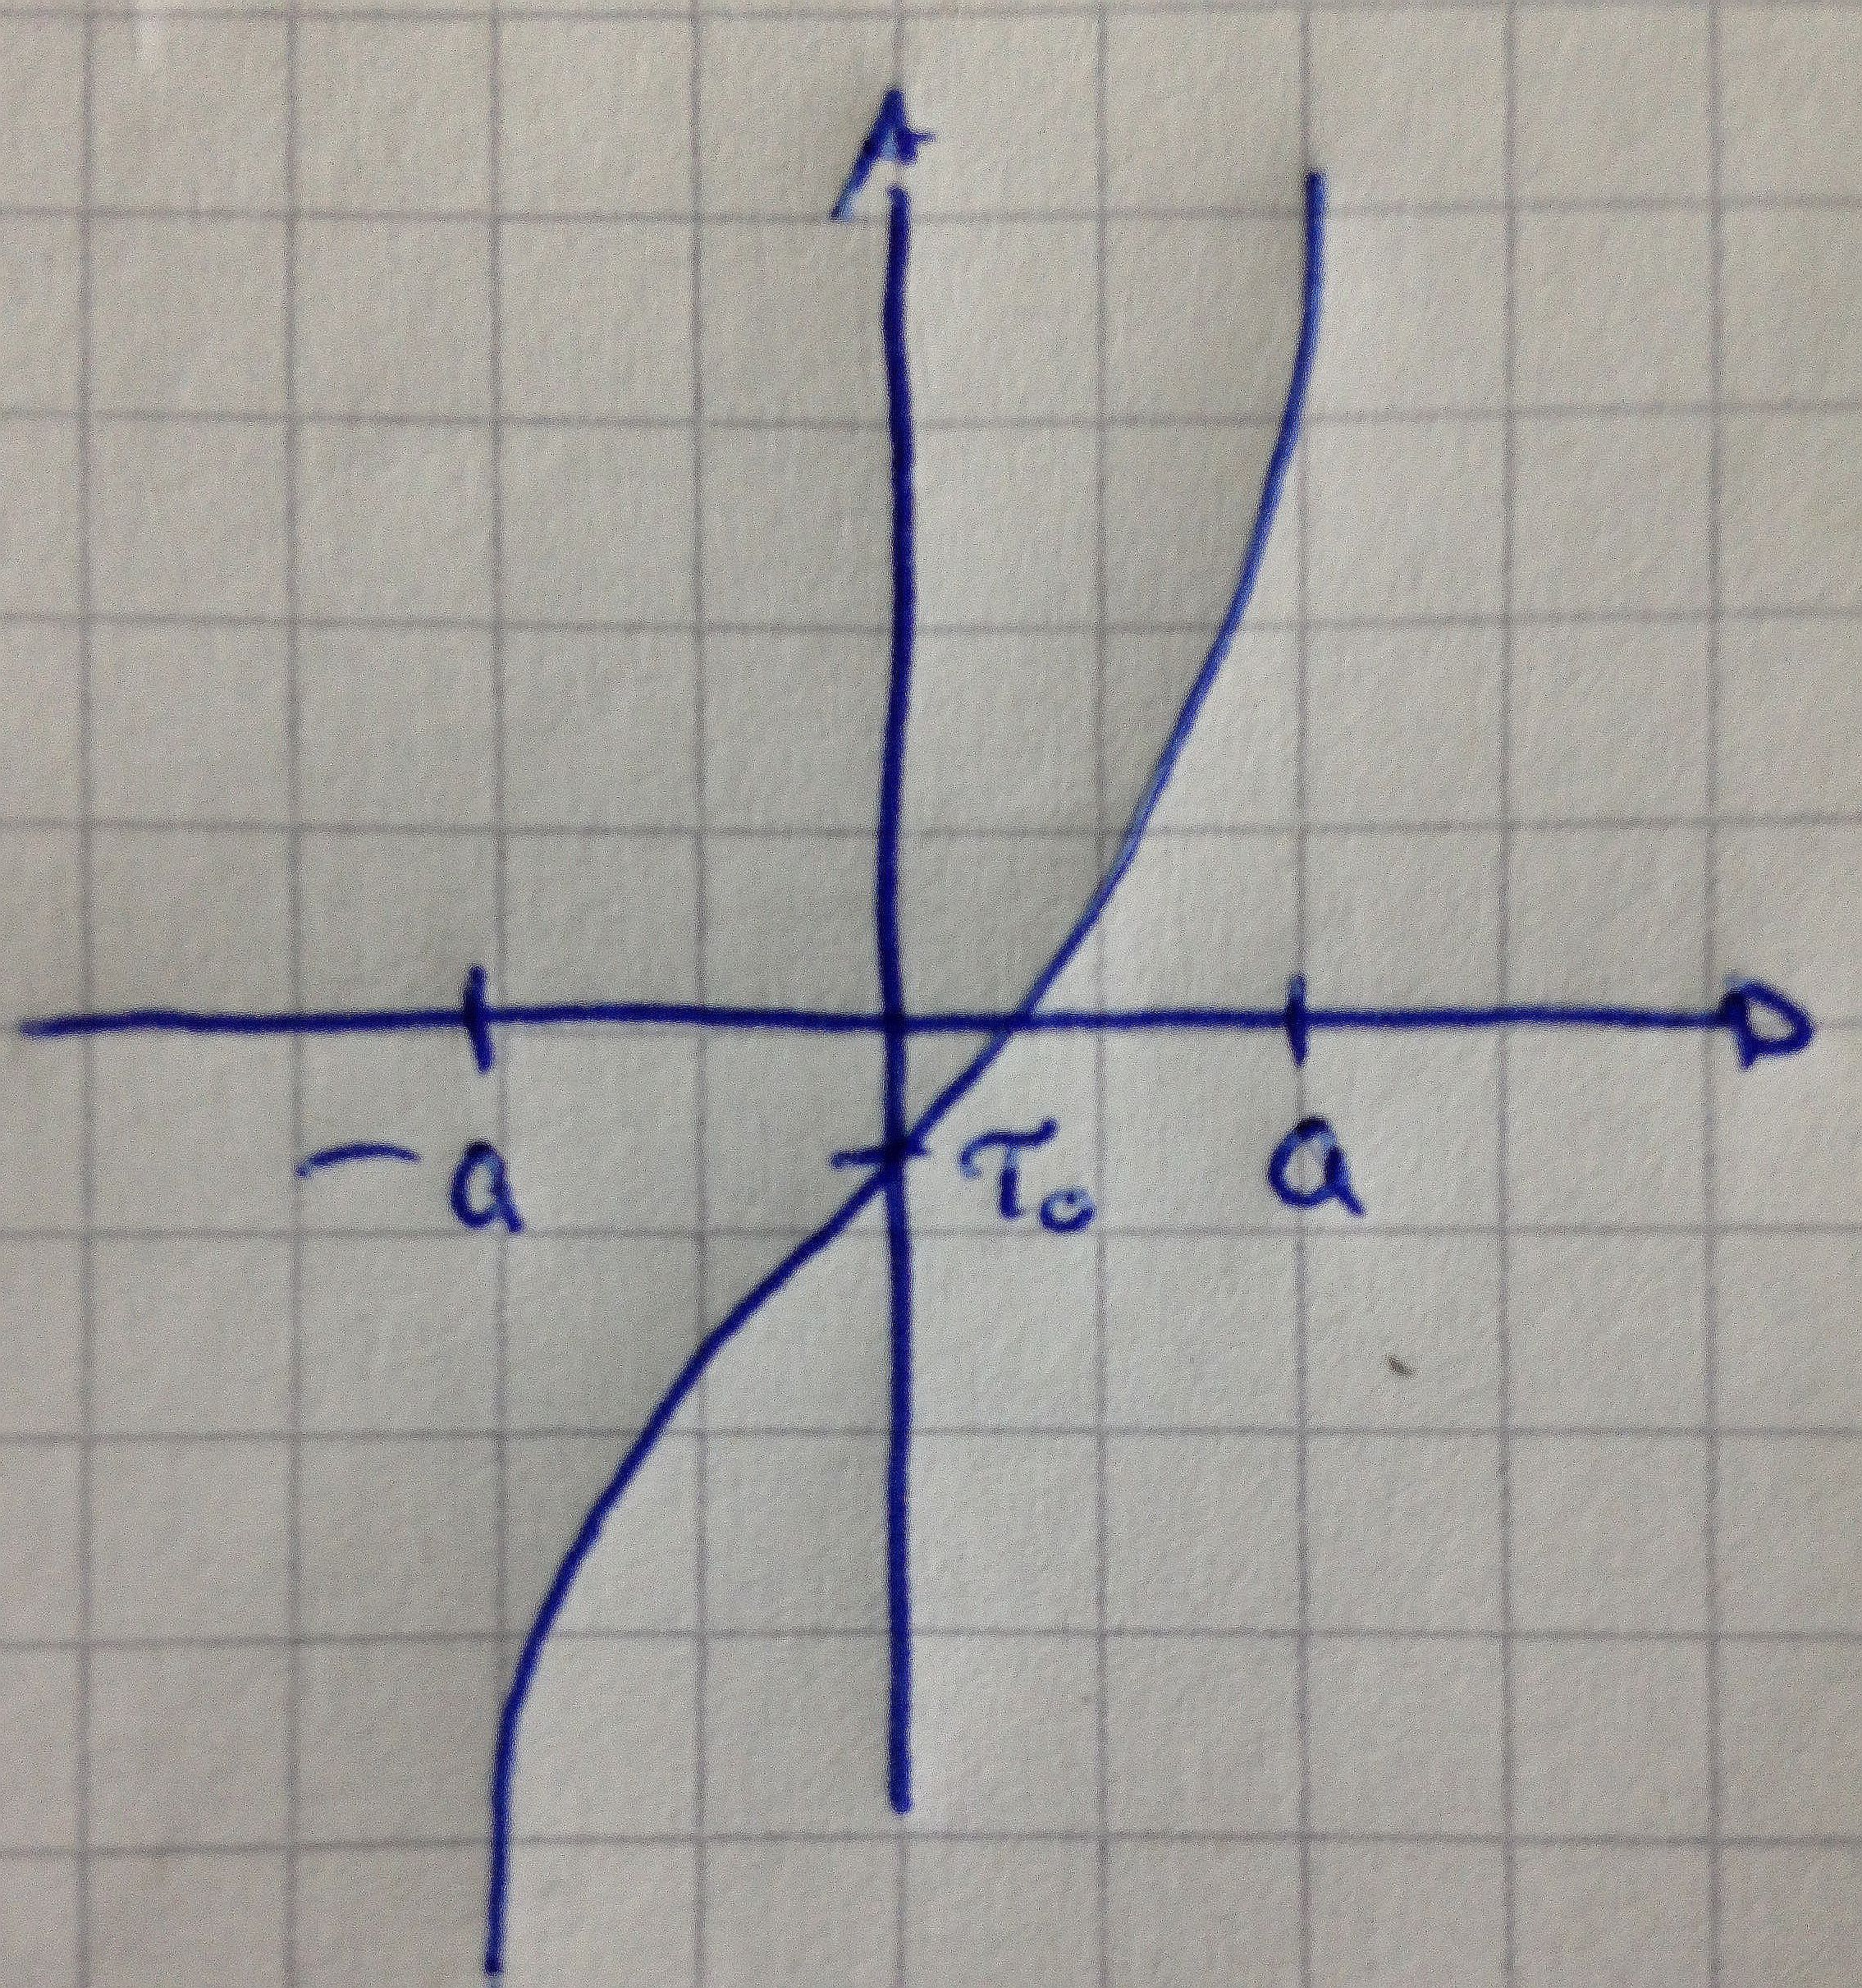
\includegraphics[width= 0.4\textwidth]{Tunneln_durch_eine_Potentialbarriere5}
		\end{center}
	\end{figure}
\FloatBarrier
	\begin{align*}
		\Delta E &= -2 \braket{+ | H | -} \sim \int [\diff x] e^{-S_E[x]}
	\end{align*}
Semiklassische Näherung: Nehme klassische Pfade und addiere Fluktuationen um klassische Pfade: 
	\begin{align*}
		x(\tau) &= x_c(\tau) + y(\tau) \\
		\frac{\delta S_E}{\delta x_c(\tau)} &= 0
		&\Rightarrow m \ddot{x}_c = V' (x_c) 
	\end{align*}
kein Minus wegen der euklidischen Zeit. Wie Newton-Bewegungsgleichung, aber mit $V \mapsto -V$
\FloatBarrier
	\begin{figure} [h]
		\begin{center}
			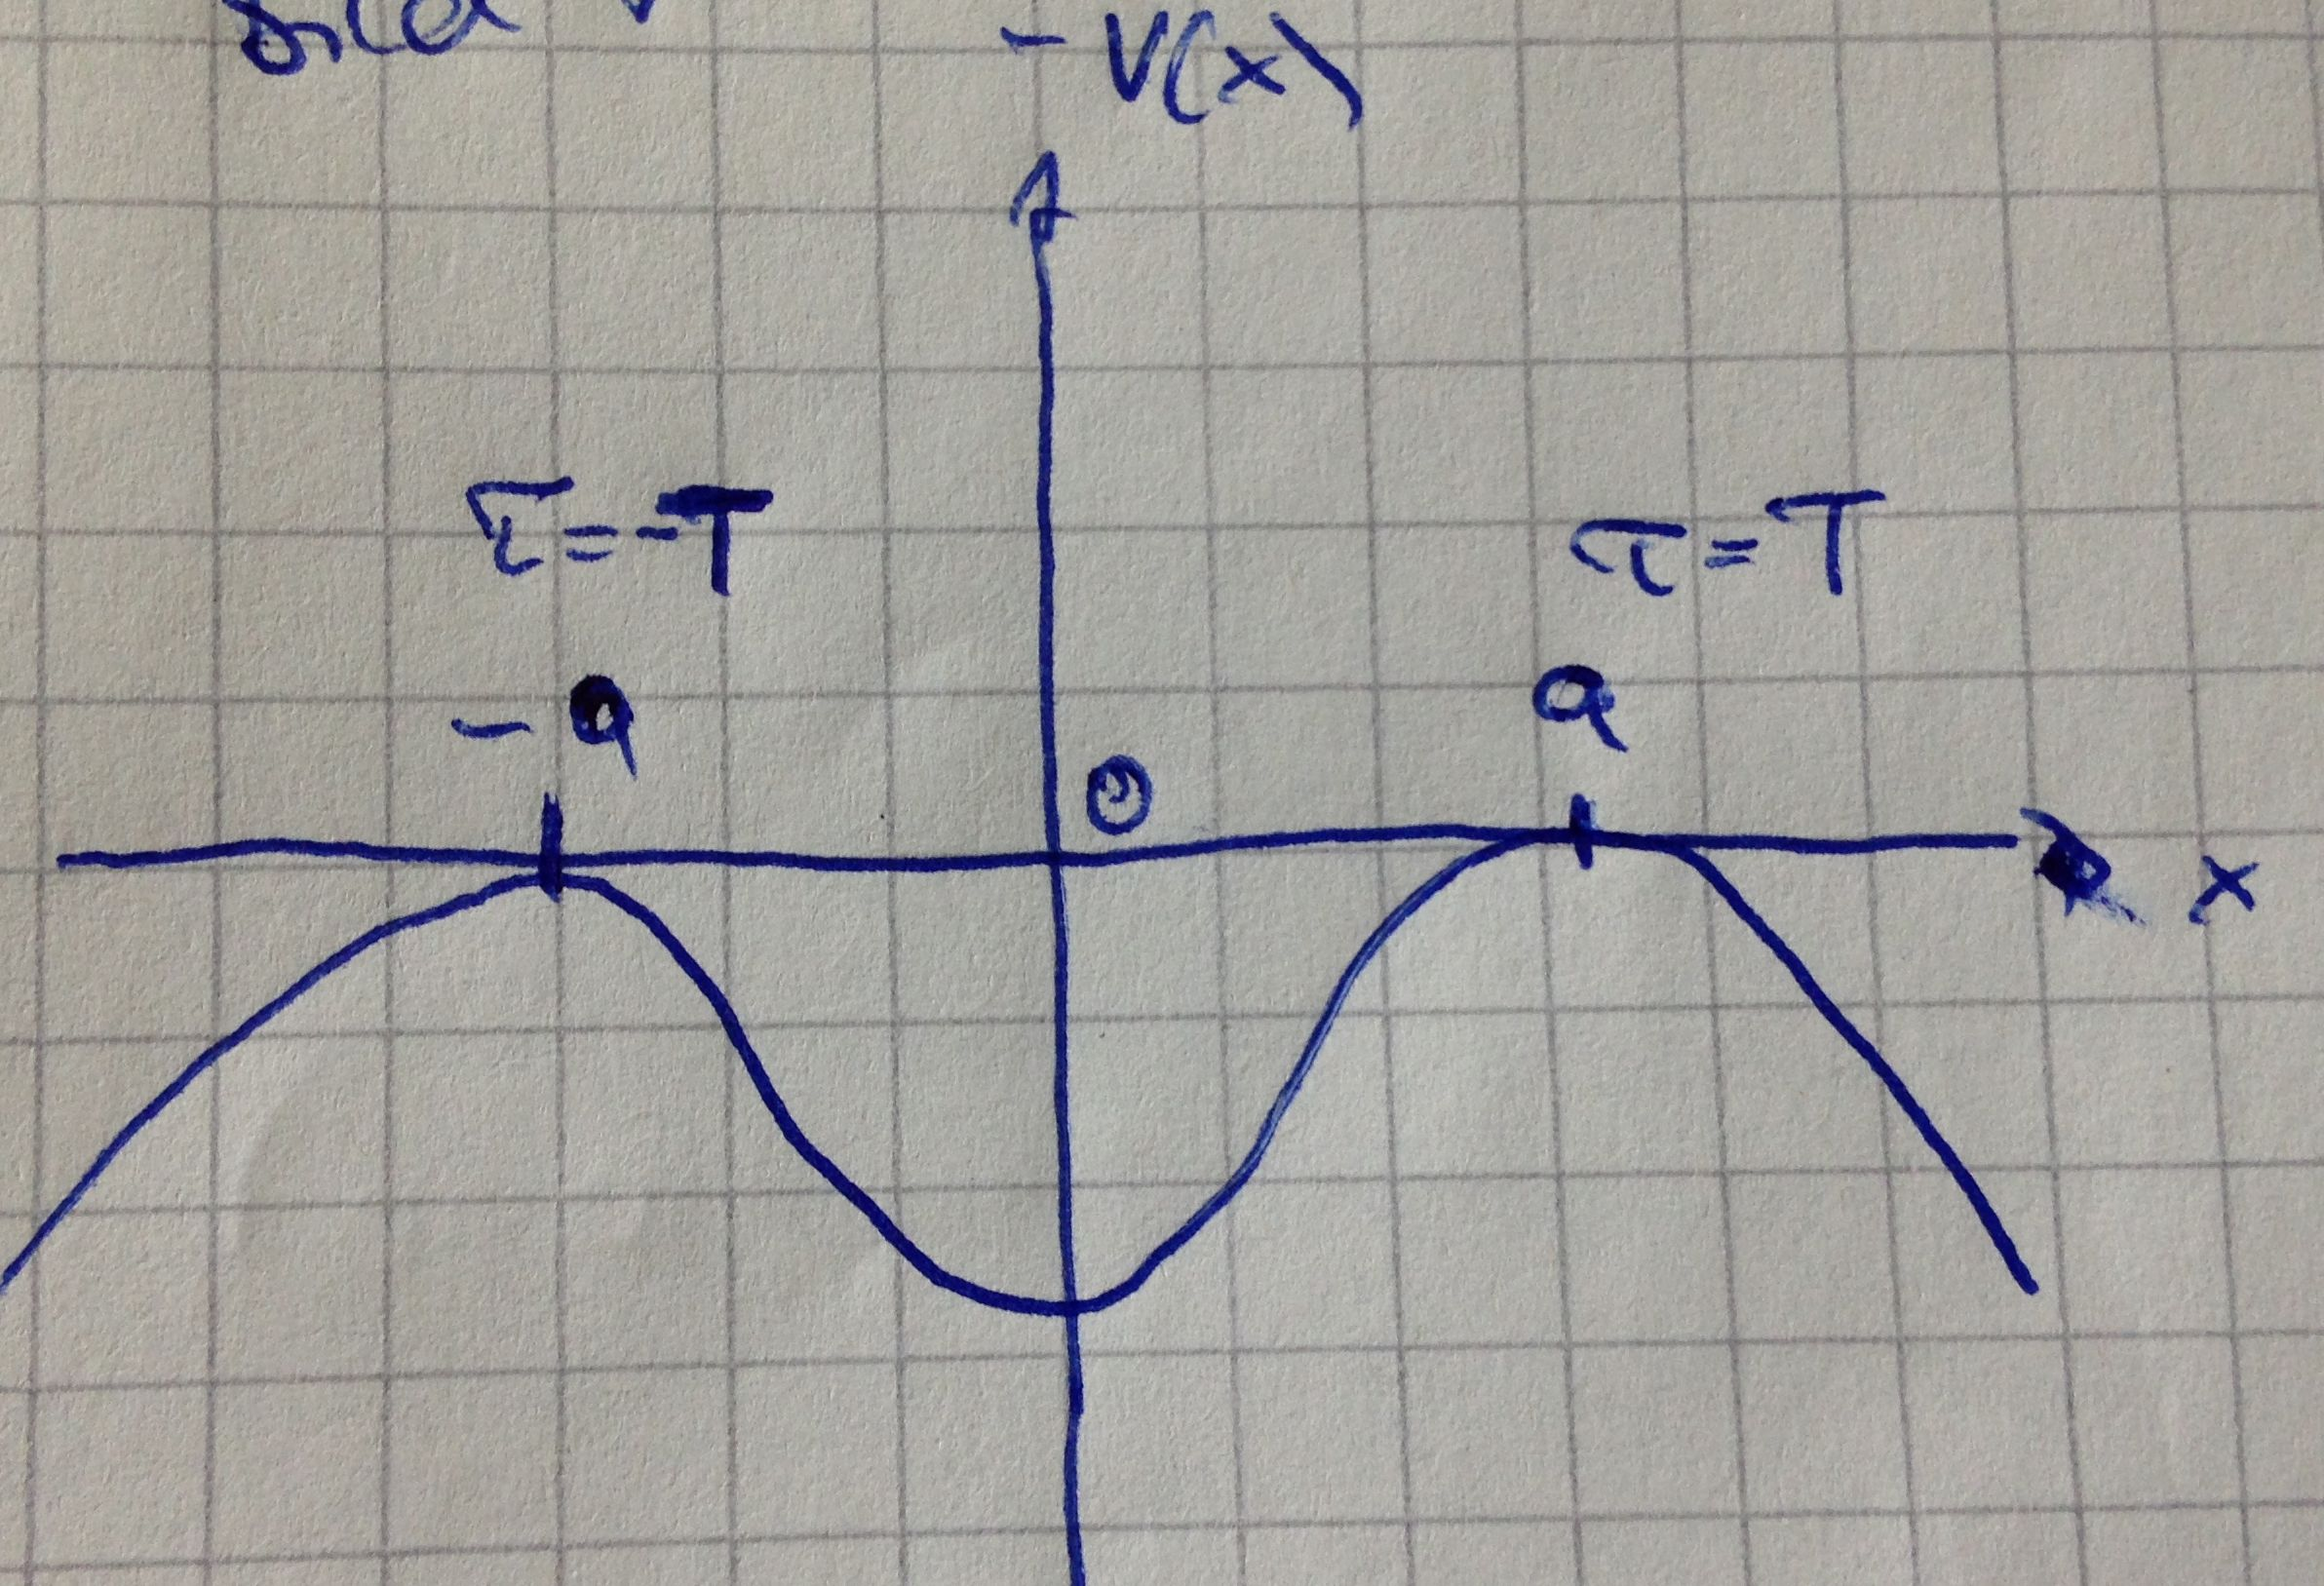
\includegraphics[width= 0.5\textwidth]{Tunneln_durch_eine_Potentialbarriere6}
		\end{center}
	\end{figure}
\FloatBarrier
	\begin{align*}
		\mathrm{T} \rightarrow \infty &: 
		x_c(\tau) = a \tanh \left[\frac{\omega}{2} (\tau- \tau_0)\right] \\
		m \omega^2 &= V^{''}(a) = 8 \lambda a^2
		\Rightarrow a^2 = \frac{m \omega^2}{8 \lambda}
	\end{align*}
je größer $\lambda$ desto ``eckiger'' wird der Pfad bei $\tau_0$ 
\\

$\omega$ klein ($\lambda a^2$ klein)
	\begin{figure} [h]
		\begin{center}
			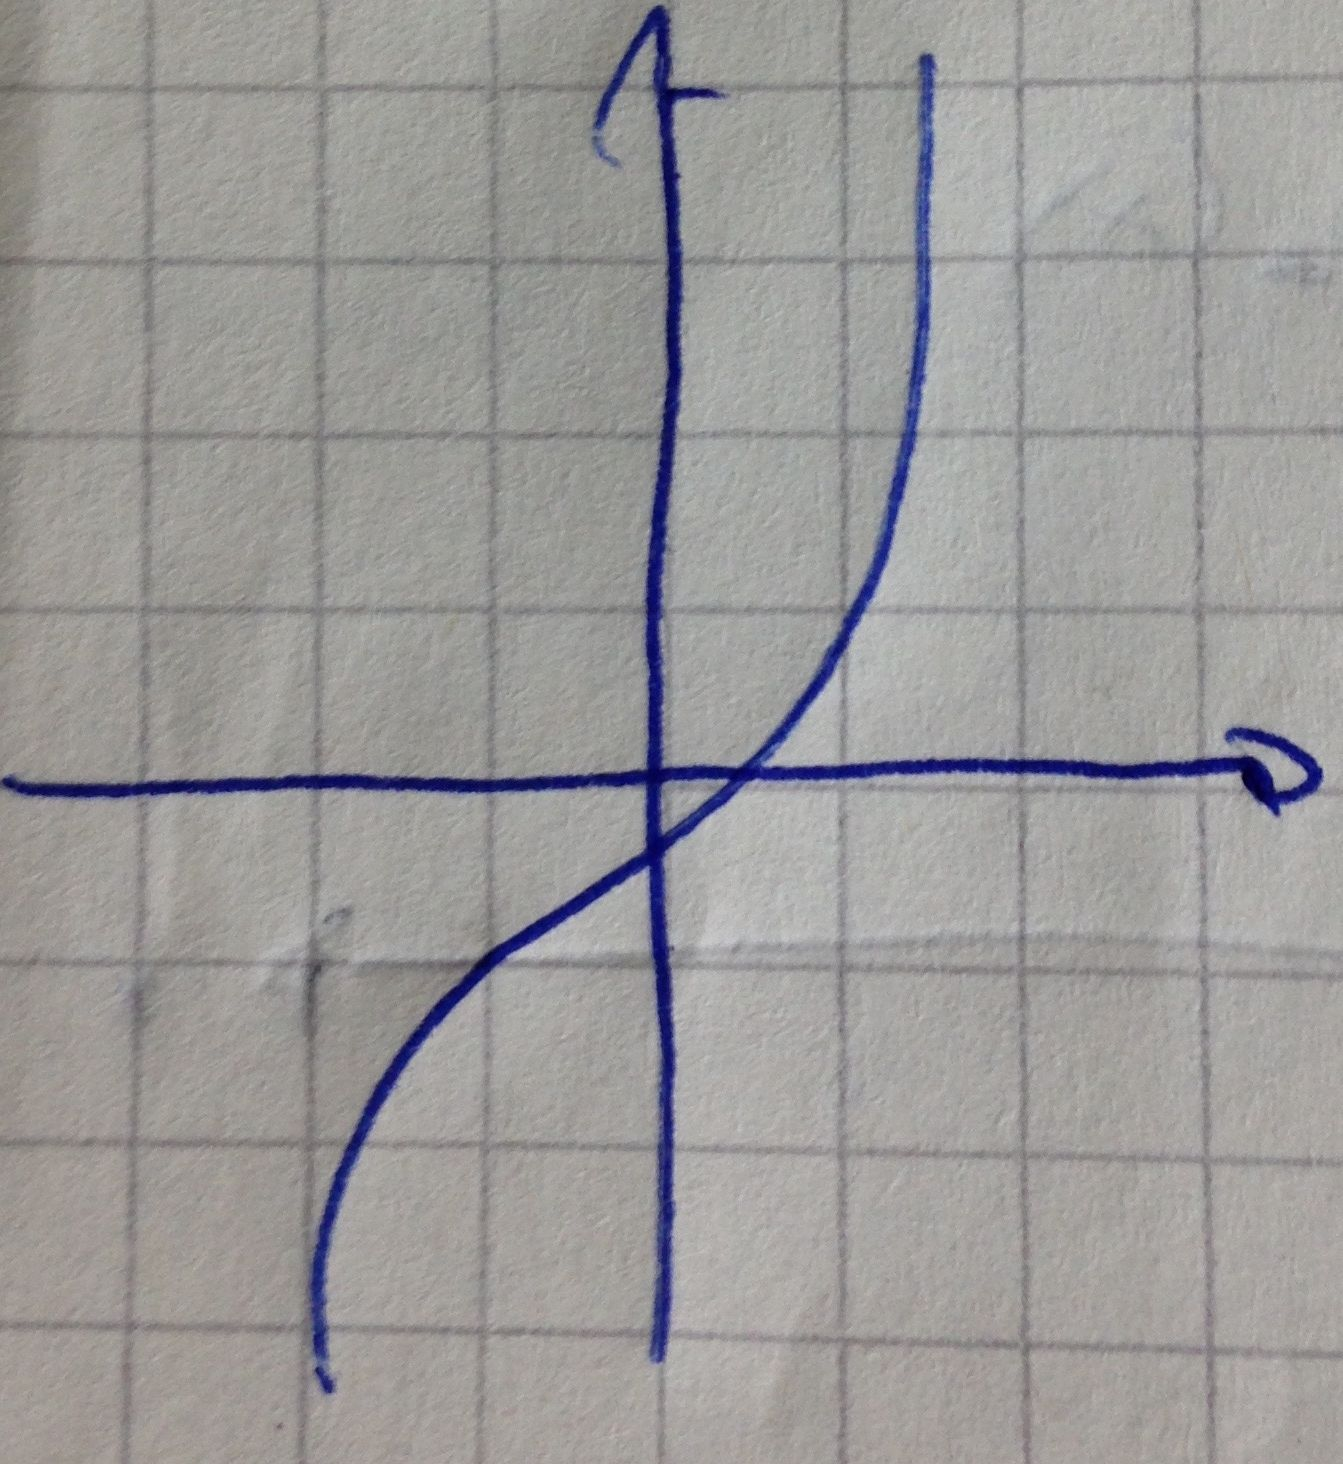
\includegraphics[width= 0.4\textwidth]{Tunneln_durch_eine_Potentialbarriere7}
		\end{center}
	\end{figure}
\FloatBarrier		
$\omega$ groß
	\begin{figure} [h]
		\begin{center}
			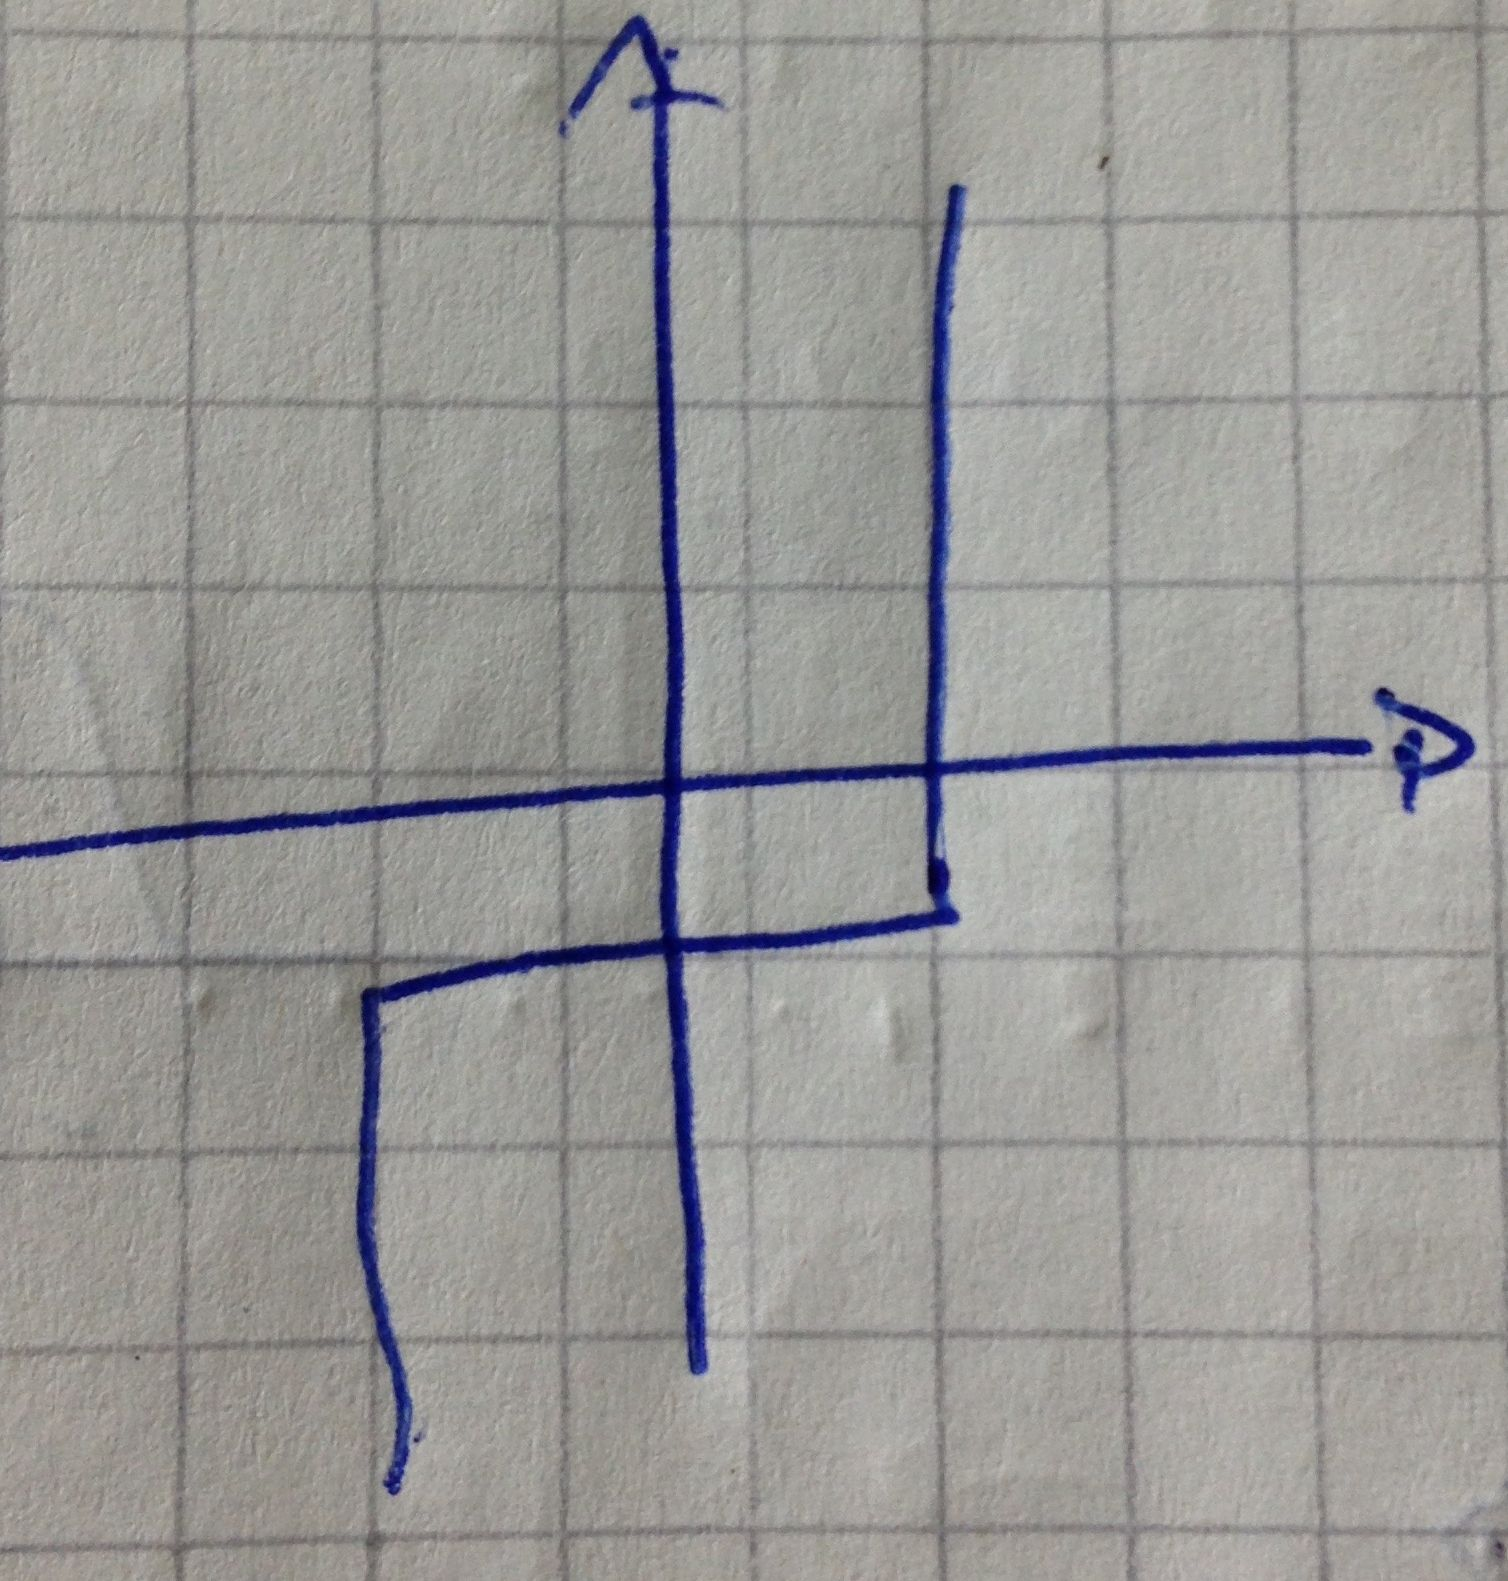
\includegraphics[width= 0.4\textwidth]{Tunneln_durch_eine_Potentialbarriere8}
		\end{center}
	\end{figure} 
\FloatBarrier
Kink (Knick) Lösung
	\begin{align*}
		\frac{m}{2} \dot{x}^2 - V(x) &= 0 
	\end{align*}
(euklidische Energieerhaltung)
	\begin{align*}
		S_E[x_c] &= \int\limits_{-\infty}^{\infty} \diff \tau
		\left[\frac{m}{2} \dot{x}^2 + V(x(\tau))\right] = \\
		&=\int \limits_{-\infty}^\infty \diff \tau m\dot{x}^2
		= \int \limits_{-a}^a \diff x m \dot{x}
		= \int \limits_{-a}^a \diff x \sqrt{2m V(x)} \\
		S_E[x_c] &= \frac{m^2 \omega^2}{12 \lambda} = \frac{4}{3} \sqrt{2m\lambda} a^3
	\end{align*}
	\begin{align*}
		x(\tau) &= x_c (\tau) + y(\tau) \\
		S_E[x] &= S_E [x_c] + \frac{1}{2} \int \diff \tau_1 \diff \tau_2 
		y(\tau_1) A(\tau_1, \tau_2) y(\tau_2) + \ldots \\
		\Delta E &\sim \int [\diff x] e^{-S_E[x]} 
		\Rightarrow \Delta E \approx N e^{-S_E[x_c]} (\det(A))^{-\frac{1}{2}} \\
		\Delta E &\approx K \underbrace{e^{- \int_{-a}^{a} \diff x \sqrt{2m V(x)}}}_{\mathclap{\text{Gamov-Faktor}}}
		= K e^{-\frac{m^2\omega^3}{12 \lambda}} \\
		K &= \frac{N}{\sqrt{\det A}} = 2 \sqrt{\frac{m^2 \omega^5}{2 \pi \lambda}}
	\end{align*}